

\tikzset{every picture/.style={line width=0.75pt}} %set default line width to 0.75pt        

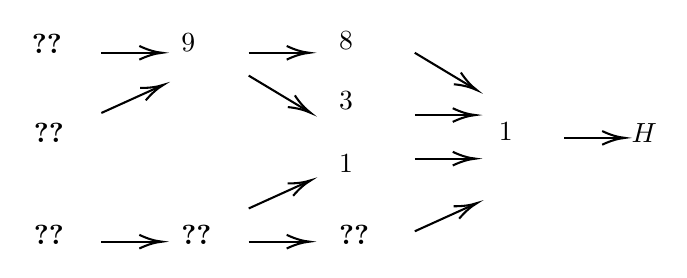
\begin{tikzpicture}[x=0.75pt,y=0.75pt,yscale=-1,xscale=1]
%uncomment if require: \path (0,273); %set diagram left start at 0, and has height of 273

%Straight Lines [id:da5524750123556669] 
\draw    (145,241) -- (172.23,241) ;
\draw [shift={(174.23,241)}, rotate = 180] [color={rgb, 255:red, 0; green, 0; blue, 0 }  ][line width=0.75]    (10.93,-3.29) .. controls (6.95,-1.4) and (3.31,-0.3) .. (0,0) .. controls (3.31,0.3) and (6.95,1.4) .. (10.93,3.29)   ;
%Straight Lines [id:da6872128650611468] 
\draw    (145,225) -- (173.18,212.23) ;
\draw [shift={(175,211.4)}, rotate = 155.61] [color={rgb, 255:red, 0; green, 0; blue, 0 }  ][line width=0.75]    (10.93,-3.29) .. controls (6.95,-1.4) and (3.31,-0.3) .. (0,0) .. controls (3.31,0.3) and (6.95,1.4) .. (10.93,3.29)   ;
%Straight Lines [id:da0006130749263758561] 
\draw    (145,150) -- (172.23,150) ;
\draw [shift={(174.23,150)}, rotate = 180] [color={rgb, 255:red, 0; green, 0; blue, 0 }  ][line width=0.75]    (10.93,-3.29) .. controls (6.95,-1.4) and (3.31,-0.3) .. (0,0) .. controls (3.31,0.3) and (6.95,1.4) .. (10.93,3.29)   ;
%Straight Lines [id:da43533627536051167] 
\draw    (145,161) -- (173.18,177.93) ;
\draw [shift={(174.89,178.97)}, rotate = 211.01] [color={rgb, 255:red, 0; green, 0; blue, 0 }  ][line width=0.75]    (10.93,-3.29) .. controls (6.95,-1.4) and (3.31,-0.3) .. (0,0) .. controls (3.31,0.3) and (6.95,1.4) .. (10.93,3.29)   ;
%Straight Lines [id:da7934755885957335] 
\draw    (74,241) -- (101.23,241) ;
\draw [shift={(103.23,241)}, rotate = 180] [color={rgb, 255:red, 0; green, 0; blue, 0 }  ][line width=0.75]    (10.93,-3.29) .. controls (6.95,-1.4) and (3.31,-0.3) .. (0,0) .. controls (3.31,0.3) and (6.95,1.4) .. (10.93,3.29)   ;
%Straight Lines [id:da8668139498353136] 
\draw    (74,150) -- (101.23,150) ;
\draw [shift={(103.23,150)}, rotate = 180] [color={rgb, 255:red, 0; green, 0; blue, 0 }  ][line width=0.75]    (10.93,-3.29) .. controls (6.95,-1.4) and (3.31,-0.3) .. (0,0) .. controls (3.31,0.3) and (6.95,1.4) .. (10.93,3.29)   ;
%Straight Lines [id:da5424771474656835] 
\draw    (74,179) -- (102.18,166.23) ;
\draw [shift={(104,165.4)}, rotate = 155.61] [color={rgb, 255:red, 0; green, 0; blue, 0 }  ][line width=0.75]    (10.93,-3.29) .. controls (6.95,-1.4) and (3.31,-0.3) .. (0,0) .. controls (3.31,0.3) and (6.95,1.4) .. (10.93,3.29)   ;
%Straight Lines [id:da3966352153586413] 
\draw    (225,236) -- (253.18,223.23) ;
\draw [shift={(255,222.4)}, rotate = 155.61] [color={rgb, 255:red, 0; green, 0; blue, 0 }  ][line width=0.75]    (10.93,-3.29) .. controls (6.95,-1.4) and (3.31,-0.3) .. (0,0) .. controls (3.31,0.3) and (6.95,1.4) .. (10.93,3.29)   ;
%Straight Lines [id:da5722514741094756] 
\draw [color={rgb, 255:red, 0; green, 0; blue, 0 }  ,draw opacity=1 ]   (297,191) -- (324.23,191) ;
\draw [shift={(326.23,191)}, rotate = 180] [color={rgb, 255:red, 0; green, 0; blue, 0 }  ,draw opacity=1 ][line width=0.75]    (10.93,-3.29) .. controls (6.95,-1.4) and (3.31,-0.3) .. (0,0) .. controls (3.31,0.3) and (6.95,1.4) .. (10.93,3.29)   ;
%Straight Lines [id:da3688731427371259] 
\draw    (225,150) -- (241.82,160.11) -- (253.18,166.93) ;
\draw [shift={(254.89,167.97)}, rotate = 211.01] [color={rgb, 255:red, 0; green, 0; blue, 0 }  ][line width=0.75]    (10.93,-3.29) .. controls (6.95,-1.4) and (3.31,-0.3) .. (0,0) .. controls (3.31,0.3) and (6.95,1.4) .. (10.93,3.29)   ;
%Straight Lines [id:da5671748893328981] 
\draw [color={rgb, 255:red, 0; green, 0; blue, 0 }  ,draw opacity=1 ]   (225,180) -- (252.23,180) ;
\draw [shift={(254.23,180)}, rotate = 180] [color={rgb, 255:red, 0; green, 0; blue, 0 }  ,draw opacity=1 ][line width=0.75]    (10.93,-3.29) .. controls (6.95,-1.4) and (3.31,-0.3) .. (0,0) .. controls (3.31,0.3) and (6.95,1.4) .. (10.93,3.29)   ;
%Straight Lines [id:da3745402223738147] 
\draw [color={rgb, 255:red, 0; green, 0; blue, 0 }  ,draw opacity=1 ]   (225,201) -- (252.23,201) ;
\draw [shift={(254.23,201)}, rotate = 180] [color={rgb, 255:red, 0; green, 0; blue, 0 }  ,draw opacity=1 ][line width=0.75]    (10.93,-3.29) .. controls (6.95,-1.4) and (3.31,-0.3) .. (0,0) .. controls (3.31,0.3) and (6.95,1.4) .. (10.93,3.29)   ;

% Text Node
\draw (187,138.4) node [anchor=north west][inner sep=0.75pt]    {$\PPIIIprn{8}$};
% Text Node
\draw (187,167.4) node [anchor=north west][inner sep=0.75pt]    {$\PPIVn{3}$};
% Text Node
\draw (187,197.4) node [anchor=north west][inner sep=0.75pt]    {$\PPIIIprn{1}$};
% Text Node
\draw (187,231.4) node [anchor=north west][inner sep=0.75pt]    {\ref{eq:P4_1_m2}};
% Text Node
\draw (111,139.4) node [anchor=north west][inner sep=0.75pt]    {$\PPVn{9}$};
% Text Node
\draw (111,231.4) node [anchor=north west][inner sep=0.75pt]    {\ref{eq:P5_2}};
% Text Node
\draw (39,139.4) node [anchor=north west][inner sep=0.75pt]    {\ref{eq:P6_7}};
% Text Node
\draw (40,182.4) node [anchor=north west][inner sep=0.75pt]    {\ref{eq:P6_4}};
% Text Node
\draw (40,231.4) node [anchor=north west][inner sep=0.75pt]    {\ref{eq:P6_2}};
% Text Node
\draw (264,182.4) node [anchor=north west][inner sep=0.75pt]    {$\PPIIn{1}$};
% Text Node
\draw (328,182.4) node [anchor=north west][inner sep=0.75pt]    {$\PIn{H}$};


\end{tikzpicture}
